\section{Introduction}

The Mars rover Opportunity’s robotic arm first stalled on November 25, 2005; its shoulder joint experienced intermittent motor stalls for years, managed with voltage workarounds and revised stow procedures. Similarly, Curiosity’s drill paused sampling for roughly eighteen months until a hand-designed drilling method restored coring \cite{nasa_science_first_drilled_sample_2018, jpl_opportunity_shoulder_2008}. Cases like these underscore that failures in continuously operating systems are inevitable \cite{factory_efficiency_2020}. Prevailing safety standards mandate \textsl{fail-freeze} behavior, requiring robots to halt when faults are detected \cite{ISO10218-1, ISO13849-1, IEC60204-1}. The result is prolonged downtime and reduced autonomy. 
In this work, we contrast this overly conservative approach with \textsl{fail-active} behavior, a more ambitious (and harder to achieve) reliability goal in which robots maintain functionality, full or reduced, under fault conditions \cite{aero_reliability}. \textbf{Fail-active behavior is how humans operate}: we continue walking on a sprained ankle, writing with a non-dominant hand, going to work when we’ve had our hearts broken. Importantly, achieving fail-active behavior comes with additional complexity. Faults reshape what the robot can physically do: actuation failures (e.g., joint range and velocity restrictions) shrink the feasible workspace and degrade manipulability, electrical faults (e.g., brownouts) reduce control authority, sensor drift can distort state estimates, and end-effector wear (e.g. lowered friction) degrades contact mechanics. Ultimately, these physical changes mean the robot can no longer move the way it originally planned.
%\ar{maybe here say soemthing like why this is hard? I mean, just adopting the word won't cut it right? }

\begin{figure}
    \centering
    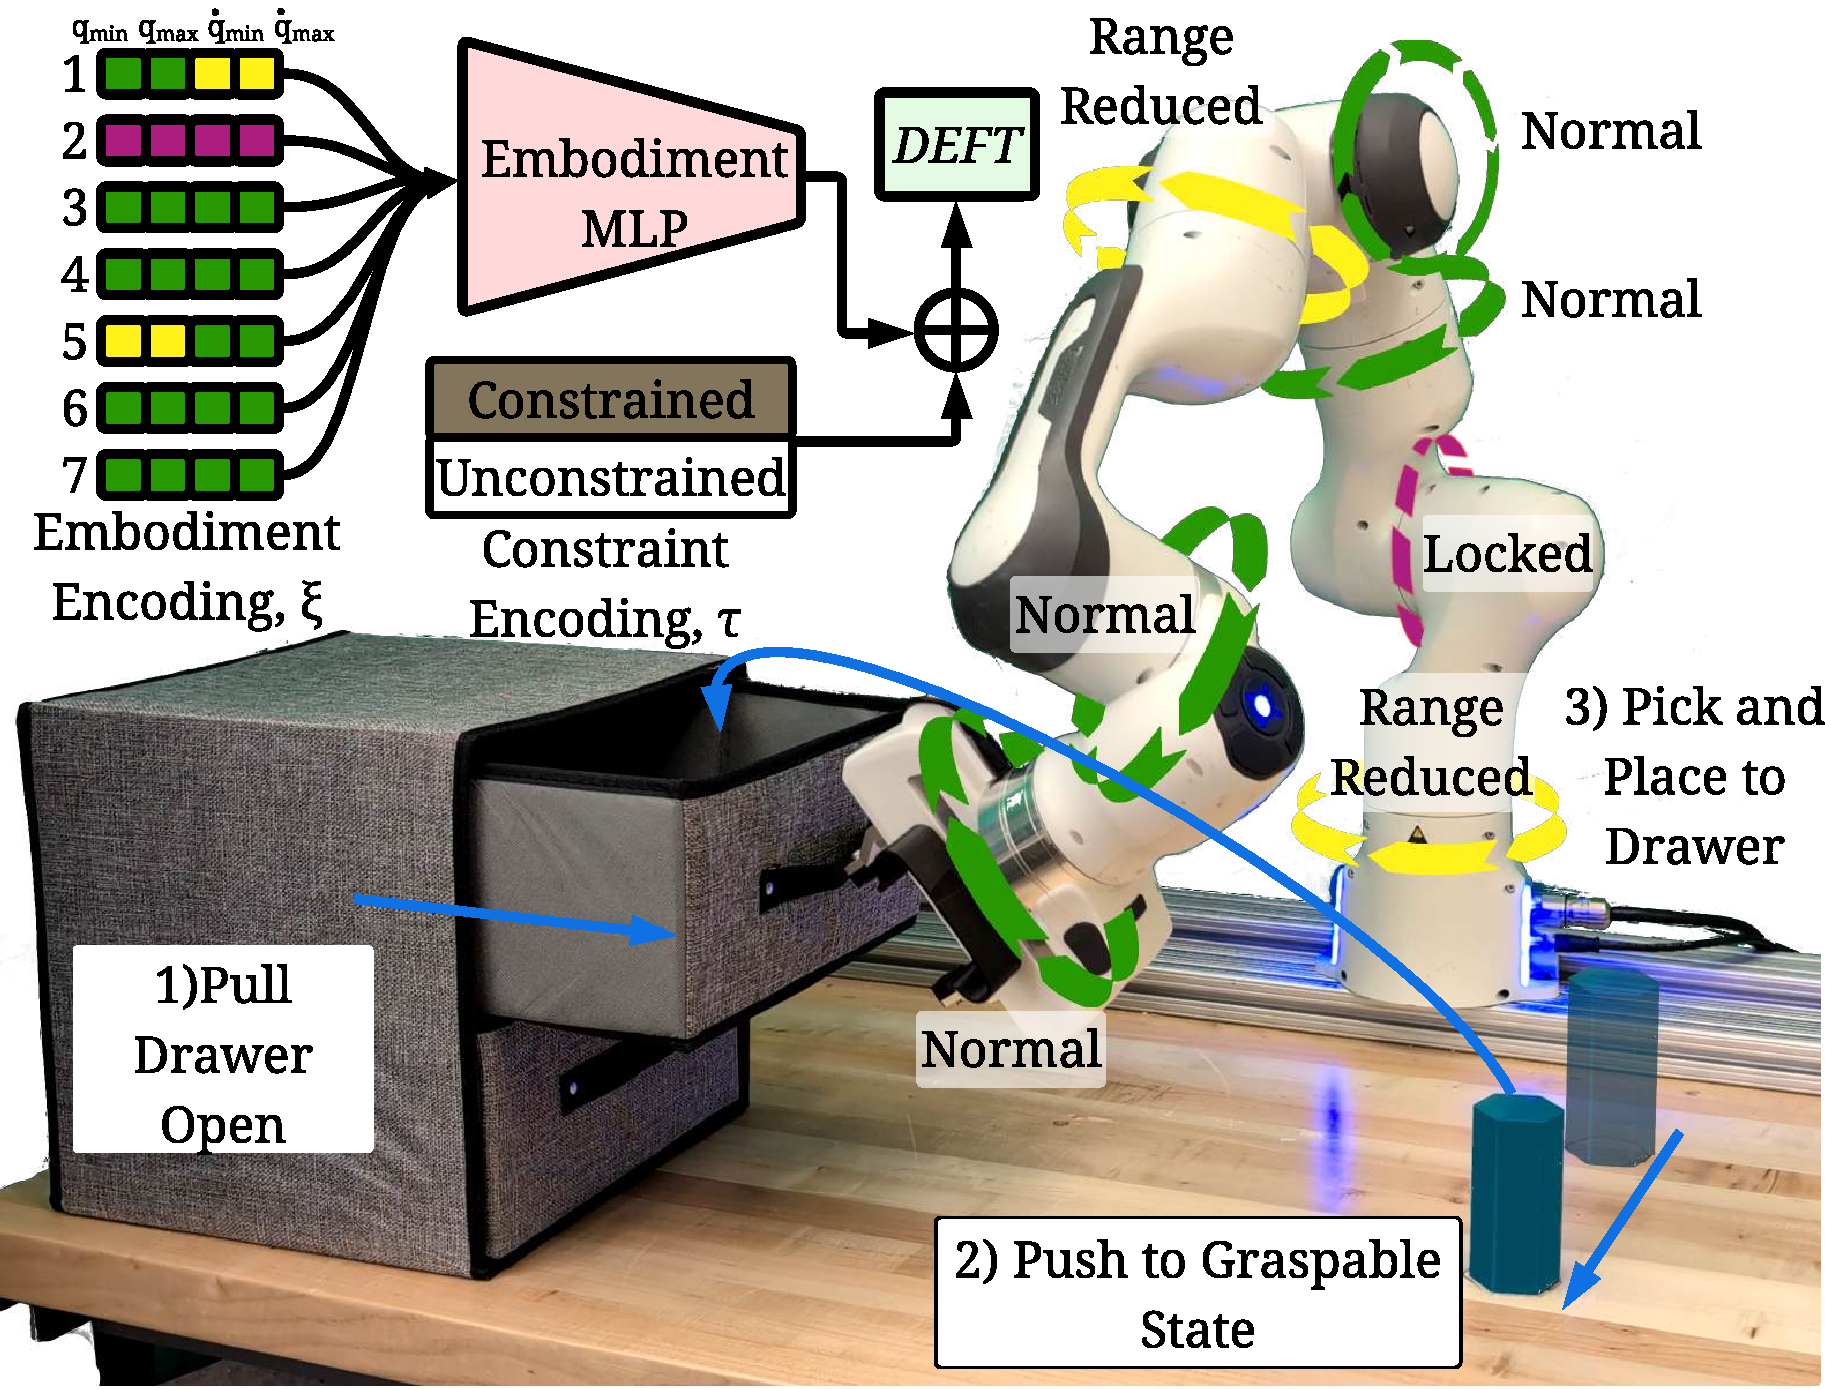
\includegraphics[width=\columnwidth]{figures/first_page_figure_compressed.pdf }
    \caption{DEFT takes as input a structured embodiment encoding representing joint-level failures and a constraint encoding then synthesizes a feasible robot trajectory via a diffusion model. After experiencing a failure, a given task will likely need to be completed in a different manner. In this figure, the pick-and-place segment is no longer feasible, given the failure condition of a locked second joint and reduced velocity range on joint 1 and reduced angle range on joint 5, and the robot must now push the object to a graspable state to complete the task. \vspace{-10pt}}
    \label{fig:first}
\end{figure}



In this work, we focus on \textit{actuation failures} as they directly affect how the robot moves. \textit{Fail-active} operation requires adapting to these altered kinematics, which can cause end-effector motion to become non-holonomic; meaning the same control input may no longer yield the same end–effector motion \cite{Bloch_Krishnaprasad_Murray_2016}. 
%
It is also important to note that since degradation can evolve over time \cite{barbieri2015sensor} and the failure state is not known a priori, \textbf{the space of failure modes is effectively unbounded}. Moreover, each joint can fail independently in multiple ways, and this complexity scales combinatorially with the robot’s degrees of freedom, \textbf{making reliable performance across failures hard to engineer}.

As failure-induced constraints redefine the robot's workspace, manipulability, and feasible interactions with the world, \textsl{we posit that each failure mode can be interpreted as a new embodiment}.  
% \ar{add a filler that describes why and what this means}
% We posit that failure could be interpreted as an embodiment shift: \ar{describe}
% Further, under embodiment shifts introduced by failure, 
% \ar{then, transition into multi-skill behaviors}
% \ar{under this lens, if you have differnet embodiments, not the same embodiment can perform that same tasks}, so
Through this lens, different embodiments are unable to perform the same tasks using the same behaviors. As no same set of behaviors can span all embodiments, multiple motion primitives are needed to expand the feasible action space and reachable task-space \cite{briscoe2024exploring}.
%so maintaining performance requires switching behaviors . 
For example, in \cref{fig:first}, reduced ranges on two joints and one locked joint prevents the robot from grasping the object. However, first pushing the object into a graspable pose and then picking-and-placing it inside the drawer, makes the task feasible.


% To this end, we must utilize motion primitives. Primitives provide compact, task aligned structure that encodes the right constraints for each family (e.g., free–space transfer vs. contact–guided alignment), and enables rapid switching when failures shrink workspace or alter feasible contacts. 

%Despite its importance, building fail-active robots is under-explored. 
Synthesizing effective motion primitives for arbitrary failure conditions is challenging due to the complex relationship between robot embodiment constraints and feasible task-space behaviors. Existing approaches fall short in three key gaps: 1) they do not generalize to arbitrary failure configurations \cite{briscoe2024exploring, xie2021maximizing}; 2) they are not capable of completing multiple manipulation primitives \cite{pham2024adaptive}; and 3) they do not address multi-joint failures \cite{mu2016kinematic, kim2024quadrupedal}. To the best of the authors’ knowledge, no existing work bridges all three of these gaps simultaneously. 
%\ar{why is it hard to address all 3 concerns simultaneously?}
Under the interpretation of failure as embodiment shift, these capabilities have not been realized as there are potentially infinite embodiments to generalize across and each embodiment has its own distribution of actions capable of achieving a set task. 
%The motion primtives combined with the infinite space of actuation failures results in a complex and multimodal trajectory distribution. 
% Diffusion models are well suited to such settings, capturing the distributions and retaining them when generating the trajectories.
Diffusion models are uniquely suited to solve this. Because they excel at modeling multimodal data distributions, diffusion policies can generate across the range of actions required to span these infinite embodiments at inference.

To this end, we present \textit{DEFT}: a \textit{D}iffusion-based \textit{E}mbodiment-aware \textit{F}ail-active \textit{T}ask-conditioned trajectory generation framework, capable of maintaining robot manipulation functionality under failure conditions. Our contributions are:
(i) an \textit{embodiment vector} encoding per-joint actuation failures for online adaptation to previously unseen failure-induced embodiments and
(ii) a \textit{constraint encoding} selecting between constrained and unconstrained motions to enable the use of multiple motion primitives.
%The conditioning on the primitive helps us push diffusion policy to the correct modes. 
Furthermore, we utilize start–goal inpainting and output clamping to enforce embodiment failure conditions \cite{repaint_lugmayr_2022}.
%the conditioned model achieves robust performance in real world scenarios. 
This allows \textsl{DEFT} to: 1) generalize to arbitrary failure configurations; 2) complete multiple manipulation primitives; and 3) handle multi-joint failures.
% We benchmark DEFT against conventional motion planning approaches, showing significant improvement in trajectory generation with arbitrary failures, obeying primitive constraints in the generated motion, and generalization to out-of-distribution failures.
We benchmark DEFT against conventional and learning based motion-planning approaches and demonstrate significant improvements in trajectory generation under arbitrary failures (up to 84\% success), adherence to task constraints (up to 78\% success), and generalization to previously unseen failures (up to 99\% success). Collectively, these results enable reliable fail-active operation, allowing robots to maintain functionality and safely complete tasks without human intervention across arbitrary failure conditions.

\vspace{-15pt}
% As deployments scale, even rare faults accumulate; \ar{<- I don't understand this} stopping for each event erodes uptime and undermines long-horizon autonomy. 
% This ability is necessary for the deployment of reliable robots, especially where intervention is costly or impossible.  
  % \ar{<- this seems a repetition of somethign you said already} 
% The number of unique robots only continues to grow exponentitially, and this growth is being buoyed by the introduction of robot motion planning polcies trained on multiple robots. Yet, one of the key challenges for their operation is the need to train or fine-tune for specific embodiments.
% Cross-embodiment policies tackle two modalities: human to robot and robot to robot. \gm{cite} However, we can define a third cross embodiment problem: failure-induced embodiment shift. Failures are inevitable over long deployments: wear, sensing drift, and partial actuation limits accumulate, altering the realized embodiment and invalidating nominal policies (\cref{applsci,mer90sols,msl_fmwi}). Human-in-the-loop recovery is slow, costly, and often impractical in remote or high-throughput settings, where downtime directly erodes mission and production value (\cref{applsci}). 
% Despite its importance, building fail-active robots is under-explored. In this work we focus on actuation failures as they are uniquely disruptive: they directly alter how the robot moves. Such joint-level failures, including reductions in angle or velocity range, cause complex and highly nonlinear changes to the mapping between control-space inputs and task-space outcomes \cite{Bloch_Krishnaprasad_Murray_2016}. Since, there exists an effectively infinite number of ways a robot can fail, and each unique failure condition may be interpreted as a new embodiment of the robot. 
% 
% % There are three key considerations of robot actuation failures: 1) degredation occurs continuously \cite{barbieri2015sensor}, 2) the failure state of the robot is not known a priori, and 3) there exists an effectively infinite number of ways a robot can fail, and each unique failure condition may be interpreted as a new embodiment of the robot. 
% 
% With the widespread development of cross-embodiment learning based approaches this natrually lends itself to the problem. But existing approaches take a train and fine-tune approach \cite{nvidia_gr00t_2025}, which requires additional expert demonstrations for the specific embodiment, or a model trained per embodiment \cite{chi2023diffusion}, or engineer in embodiment understanding \gm{cite body transformer}. These cannot address the three key considerations of actuation failure.
% Despite its importance, building fail-active robots is under-explored. We focus on actuation failures because they directly alter how the robot moves: joint-level range and velocity caps (or locks/torque limits) induce highly nonlinear changes in the mapping from control inputs to task-space outcomes \cite{Bloch_Krishnaprasad_Murray_2016}. 
% 
% \ar{again , you don't say why its' hard, you just say it's not explored} 
% \ar{need to impvover here. You want to plant the flag but you are not doing it well enough}

%conditioned explicitly on the selected motion primitive and the robot’s failure-induced embodiment constraints.

% \gm{we dance around it a lot and don't say it explicitly: We need to motivate diffusion because 'the complex relationship between
% robot embodiment constraints and feasible task-space behaviors', each mode can be viewed as a new embodiment of the robot (multimodal distributions, say this exactly), primitives also make it a multimodal distribution. }
% Conditioning on a small set of primitives reduces sample complexity, guides the denoiser toward the appropriate constraint manifold, and yields plans that remain feasible under failure–induced embodiment changes \cite{Huang2021}. 
% In practice, we use two primitives—\emph{transport} and \emph{guide}—as building blocks for varied manipulation tasks, and learn a single policy that selects and instantiates them under changing joint limits and velocities. 
% Prior work shows that enabling fail-active behavior may require robots to switch between alternative manipulation behaviors (e.g., from pick-and-place to poking or pushing), each inducing distinct classes of task-specific interactions .

% Treating each actuation fault as a morphology shift;  tightened joint limits, altered Jacobian conditioning, or partial torque loss; makes cross-embodiment methods a natural fit.

 % Viewing failure as a new embodiment suggests borrowing tools from cross-embodiment learning. However, common strategies have limitations for fault response: (i) train-then-fine-tune VLA create robot-specific policies when adapting to a new embodiment (post-training per platform) \cite{nvidia_gr00t_2025}, (ii) per-embodiment policies deliver high in-distribution reliability but offer little zero-shot transfer \cite{chi2023diffusion}, and (iii) engineered embodiment understanding (e.g., representation alignment) can improve transfer yet still presumes a stable morphology rather than a drifting failure state \cite{wiut24}.

% \ar{again, you don' say what  you do}
% \gm{explicitly what we do is diffusion for failure recovery and then add an additional conditionning vector to diffusion to close the sim to real gap: it's a vector of joint limits and a vector telling it whether to constrain the ee orientation and motion to a straight line or not. We need to re include primitive motivation (my prior work) and do a good job at saying why constrained motion is interesting to test}
% \gm{latest note: sim2real is hard, we got good results in sim using diffusion instead of optimization like existing approaches but gap in real world and conditioning helped close it, we did diffusion -> sim to real gap -> needed embodiment conditioning}
% Robots are becoming increasingly ubiquitous, being used in applications ranging from healthcare, to space, to high-mix warehouse automation. .facto}Current standards enforce \textsl{fail-freeze} behavior: robots must halt operation when faults are detected \cite{ISO10218-1, ISO13849-1, IEC60204-1}. 
% On Mars, months-long and even multi-year recoveries are routine. Opportunity’s robotic arm shoulder motor first stalled on November 25, 2005, prompting workarounds and continued management of intermittent stalls years later; Curiosity’s drill feed fault halted coring from December 2016 until May 2018, when a new feed extended drilling method restored sampling. These episodes illustrate that faults in continuously operating systems are inevitable \cite{factory_efficiency_2020}. Current standards enforce \textsl{fail-freeze} behavior: robots must halt operation when faults are detected \cite{ISO10218-1, ISO13849-1, IEC60204-1}. In this work, we borrow the term \textsl{fail-active} from the aerospace community as a long-term goal for robots, defined as the ability to function completely or in a reduced manner in the event of a failure \cite{aero_reliability}.  


%Robots are on the cusp of ubiquity in the real world, enabled by their growing physical ability and the success of end-to-end models that allow them to perform many tasks effectively \gm{put some good cites}. However, one major impediment to mass adoption is the inevitability of hardware failure. When a hardware fault is detected, current standards recommend that robots \textsl{fail-freeze}: stop operation when a fault is detected. \cite{ISO10218-1, ISO13849-1, IEC60204-1}  This stands in stark contrast to other mechanical systems, such as automobiles and aircraft, that are \textsl{fail-active}: able to continue to perform its function with a failure occuring. \cite{aero_reliability} The need to halt operations in robots experiencing a fault is fundamentally incompatible with use cases where continuous operation despite hardware faults is essential such as: surgical robots, space and remote robots, and future utilitarian robots.

%There are many components in a robot that can fail \gm{cite one of the old long-term study papers}, but in this work we focus on failures that affect the actuation of the joints. Failures in the joints are of particular importance because they warp the coupling of the configuration and task spaces in non-linear ways. \cite{Bloch_Krishnaprasad_Murray_2016, atreya_steering}. Joint failures can manifest in a number of ways: such as through actuator failures that limit joint velocity, acceleration, or range, or result in joint locking. Compensating for the failures is made more difficult by the near-infinite space of possible failure configurations: each joint may independently experience varying limits on position, velocity, or acceleration, and the robot must adapt through compensatory behaviors that grow combinatorially with the number of degrees of freedom. Handling such failures requires motion planning systems that solve a dual problem: 1) understanding how failure constrains trajectory generation, and 2) being aware of the requirements of the task that the robot is to complete to serve its function.

%Prior work in has shown that being fail-active to joint failures in task space necessitates the use of an expanded set of manipulation behaviors in order to complete the tasks commanded of the robot. \cite{briscoe2024exploring}. This paper will adopt this paradigm to enable fail-active task planning. Pick and place can become infeasible under certain failures, but other approaches, such as poking and pushing, can still work. 

%Each of the two prior problems consist of trajectories that belong to a unique distribution. and going across distributions is hard. Each modality of motion primitive has a unique joint trajectory distribution that forces it to be the class of motion in the end effector. Each failure changes the limits in some way that non-linearly maps to changes in the task space, so each failure for each joint for each type represents its own distribution of trajectories. Defining these constraints empirically is exceedingly difficult and infeasible, but we can learn to condition some information of the failure and of the task in order to produce trajectories in and across these distributions. Diffusion is good at this because it can learn a conditional model of trajectories given some information about the trajectory. 

%Using all this, the contributions of this work are:
%\begin{itemize}
 %   \item A definition of a more general set of failures, including full, partial, reduced velocity, and reduced acceleration, to address than any prior work
    %\item A meaure of the affect of failures have on the robot's task capability
    %\item The ability to generate failure constrainted trajectories
    %\item The ability to create task-specified actions with failures
%\end{itemize}


% To deploy robots in unstructured or remote environments over long time horizons—on the order of years—we must develop systems that can automate this graceful degradation. We define this capability as fail-active: the ability for a robot to continue operating even as its embodiment degrades, such as through actuator failures that limit joint velocity, acceleration, or range, or result in joint locking. Handling such failures requires motion planning systems that incorporate embodiment-specific constraints directly into trajectory generation.

% This challenge is made more difficult by the near-infinite space of possible failure configurations: each joint may independently experience varying limits on position, velocity, or acceleration, and the robot must adapt through compensatory behaviors that grow combinatorially with the number of degrees of freedom \gm{cite or rephrase if needed}. Despite the inherent flexibility of diffusion-based planning approaches, most prior work assumes a constant embodiment. In contrast, we embed embodiment-conditioned adaptability into a diffusion model, enabling it to generalize over multimodal distributions of joint capabilities and failure states.

% Because the relationship between control actions and joint motion becomes increasingly nonlinear under embodiment changes, diffusion models are well-suited to this problem. Just as they are able to model multiple valid solutions for complex real-world tasks, they are also capable of capturing diverse strategies for achieving a task across various physical degradations. Our approach extends this flexibility, offering a step toward scalable and resilient robot autonomy.

% For robots to remain effective over long time horizons---on the order of years---they must adapt to inevitable physical degradation. In high-stakes contexts such as space or remote exploration, maintaining operational capability is critical, as physical repairs and human intervention are infeasible\gm{cite}. 



% In this paper, we enable robots to be fail-active, defined as the ability to continue operation when the physical form of the robot degrades, in the face of actuator failures. Actuator failures, including decreased joint velocity and acceleration, reduced angle range, or full locking, requires trajectory generation approaches that incorporate these changes in the embodiment while planning for tasks \gm{cite if possible}. This difficulty is compounded by the near-infinite space of possible failure configurations, where each joint may experience varying constraints on position, velocity, and acceleration, and the compensatory degrees of freedom grow combinatorially with the complexity of the robot \gm{rewrite this sentence}. State-of-the-art failure recovery methods only address single joint failures and limited types of failures\gm{cite}. To truly enable a robot to be fail-active, the robot's motion planning system must be able to adapt to any change in the robots abilities. Without addressing this challenge, long-term autonomy in unstructured and remote environments may remain out of reach. 


% Existing work in fault-tolerant motion generation fall into three categories: 1) pre-computation, 2) analytical inverse-kinematics, and 3) learning-based methods. Pre-compuation creates a limited set of task-specific motions, which restricts their ability to adapt to new or unforeseen failure configurations \citep{briscoe2024exploring}. Approaches based on analytical inverse kinematics require hand-crafted, embodiment-specific models and are limited to single failure modes at a time \citep{mu2016kinematic, lewis1997fault}. Learning-based methods, such as reinforcement learning, have demonstrated the ability to compensate for joint impairments but are typically restricted to specific robot morphologies or failure types \citep{pham2024adaptive, kim2024quadrupedal}.  When the robot's embodiment degrades, this task and action separation creates a mismatch between planned and executed motions \gm{cite}.

% Existing methods are inadequate because they are not truly generalizable to arbitrary failures. They are unable to handle combinations or multiple types of actuator failures. The core challenge is to develop a trajectory generation model that can compensate for arbitrary failures while remaining capable of generating feasible trajectories under real-world environmental constraints. An ideal solution would take in the failure state of the robot, alongside task and environmental information, and generate valid, executable trajectories without needing retraining or post-processing. 
% Diffusion models — with their ability to model multimodal distributions and generalize across varying conditions — are particularly well-suited to address this challenge. For instance, industrial arms like the KUKA LBR iiwa are rated for approximately 30,000 hours of operation, or about 3.5 years \citep{kuka_lbr_iiwa}.

% In this paper, we introduce a diffusion-based trajectory generation framework that is explicitly conditioned on the robot's embodiment data. Diffusion models are well-suited to this problem because they can model complex, multimodal distributions — in this case, the space of feasible robot trajectories under varying kinematic constraints. The key insight is that by conditioning the diffusion model on the robot’s joint limits (position, velocity, and acceleration), the model can generate multiple feasible solutions even under unseen failure scenarios. Unlike traditional methods that require that are tailored to specific failure modes, our approach allows the model to adapt to new actuator constraints at inference time despite being trained on a finite set of failures. We adopt a diffusion policy framework \citep{chi2023diffusion} and extend it to handle embodiment conditioning by integrating two key mechanisms: (1) direct conditioning of joint angle, velocity, and acceleration limits, and (2) clamping the denoised trajectory at each diffusion step to ensure that the generated joint states remain within the specified limits. This approach enables generalization to unseen embodiments and failure modes at inference time without requiring failure-specific or task-specific retraining or separate post-processing to enforce feasibility. To the best of our knowledge, this is the first approach to successfully condition a diffusion model on actuator data to handle both kinematic and dynamic failures concurrently — including complex scenarios where joint angle and velocity limits are restricted simultaneously. We evaluate our approach over a set of basic motion primitives, demonstrating robustness over increasingly disabling failures. We further performed an ablation study to demonstrate the need for each part of the conditioing and clamping of the diffusion model \gm{do better}.



% We are on the cusp of having robots operate in the real world en masse (cite hyundai buying 10k humanoids) because they are able to do many tasks well using an end-to-end models because they are so physically complex
% An impediment to universal adoption is the enevitable failure of the hardware of the system 
% right now iso recommends stopping system when a fault occurs --- that is not scalable
% that is in stark contrast to humans that are able to compensate to complete tasks when injured
% An existing example is the mars rover arm failing quickly after 
% we want to make systems that are able to adapt and continue operating when they have degradation (graceful degradation)
% existing diffusion approaches (and motion planning at large) expect a constant embodiment, despite their inherent flexibility, we put that flexability in
% because the relationship between actions and joint motions changes non-linearly with changes in joint capability, we need to use diffusion because it can have the multimodal distribution understanding

% for the same reason they are able to handle multiple complex tasks in the real world, they are able to handle multiple system failure states to complete the same task